%!TEX TS-program = xelatex
\documentclass[]{friggeri-cv}
\usepackage{afterpage}
\usepackage{hyperref}
\usepackage{color}
\usepackage{xcolor}
\usepackage{smartdiagram}
\usepackage{fontspec}
\usepackage[export]{adjustbox}
% if you want to add fontawesome package
% you need to compile the tex file with LuaLaTeX
% References:
%   http://texdoc.net/texmf-dist/doc/latex/fontawesome/fontawesome.pdf
%   https://www.ctan.org/tex-archive/fonts/fontawesome?lang=en
%\usepackage{fontawesome}
\usepackage{metalogo}
\usepackage{dtklogos}
\usepackage[utf8]{inputenc}
\usepackage{tikz}
\usepackage{tcolorbox}
\usetikzlibrary{mindmap,shadows}
\hypersetup{
    pdftitle={},
    pdfauthor={},
    pdfsubject={},
    pdfkeywords={},
    colorlinks=false,           % no lik border color
    allbordercolors=white       % white border color for all
}
\smartdiagramset{
    bubble center node font = \footnotesize,
    bubble node font = \footnotesize,
    % specifies the minimum size of the bubble center node
    bubble center node size = 0.5cm,
    %  specifies the minimum size of the bubbles
    bubble node size = 0.5cm,
    % specifies which is the distance among the bubble center node and the other bubbles
    distance center/other bubbles = 0.1cm,
    % sets the distance from the text to the border of the bubble center node
    distance text center bubble = 0.5cm,
    % set center bubble color
    bubble center node color = pblue,
    % define the list of colors usable in the diagram
    set color list = {lightgray, materialcyan, orange, green, materialorange, materialteal, materialamber, materialindigo, materialgreen, materiallime},
    % sets the opacity at which the bubbles are shown
    bubble fill opacity = 0.6,
    % sets the opacity at which the bubble text is shown
    bubble text opacity = 0.5,
}

\addbibresource{bibliography.bib}
\RequirePackage{xcolor}
\definecolor{pblue}{HTML}{0395DE}

\begin{document}
~~~
\header{Long }{Nguyen}
      {Computer Engineer}
      
% Fake text to add separator      
\noindent\makebox[\linewidth]{\rule{\paperwidth}{3pt}}
%\fcolorbox{white}{black}{\parbox{1cm}{%
%\.
%}}

% https://tex.stackexchange.com/questions/19579/horizontal-line-spanning-the-entire-document-in-latex

%\fcolorbox{white}{black}{\parbox{\dimexpr\textwidth\fboxsep\fboxrule}{%
%\.
%}}

%\fcolorbox{white}{black}{\parbox{\dimexpr\textwidth-2\fboxsep-2\fboxrule}{%
%\_\_\_\_
%}}

% In the aside, each new line forces a line break
\begin{aside}
%scale 0.35 for long.JPG avatar-cricle
%  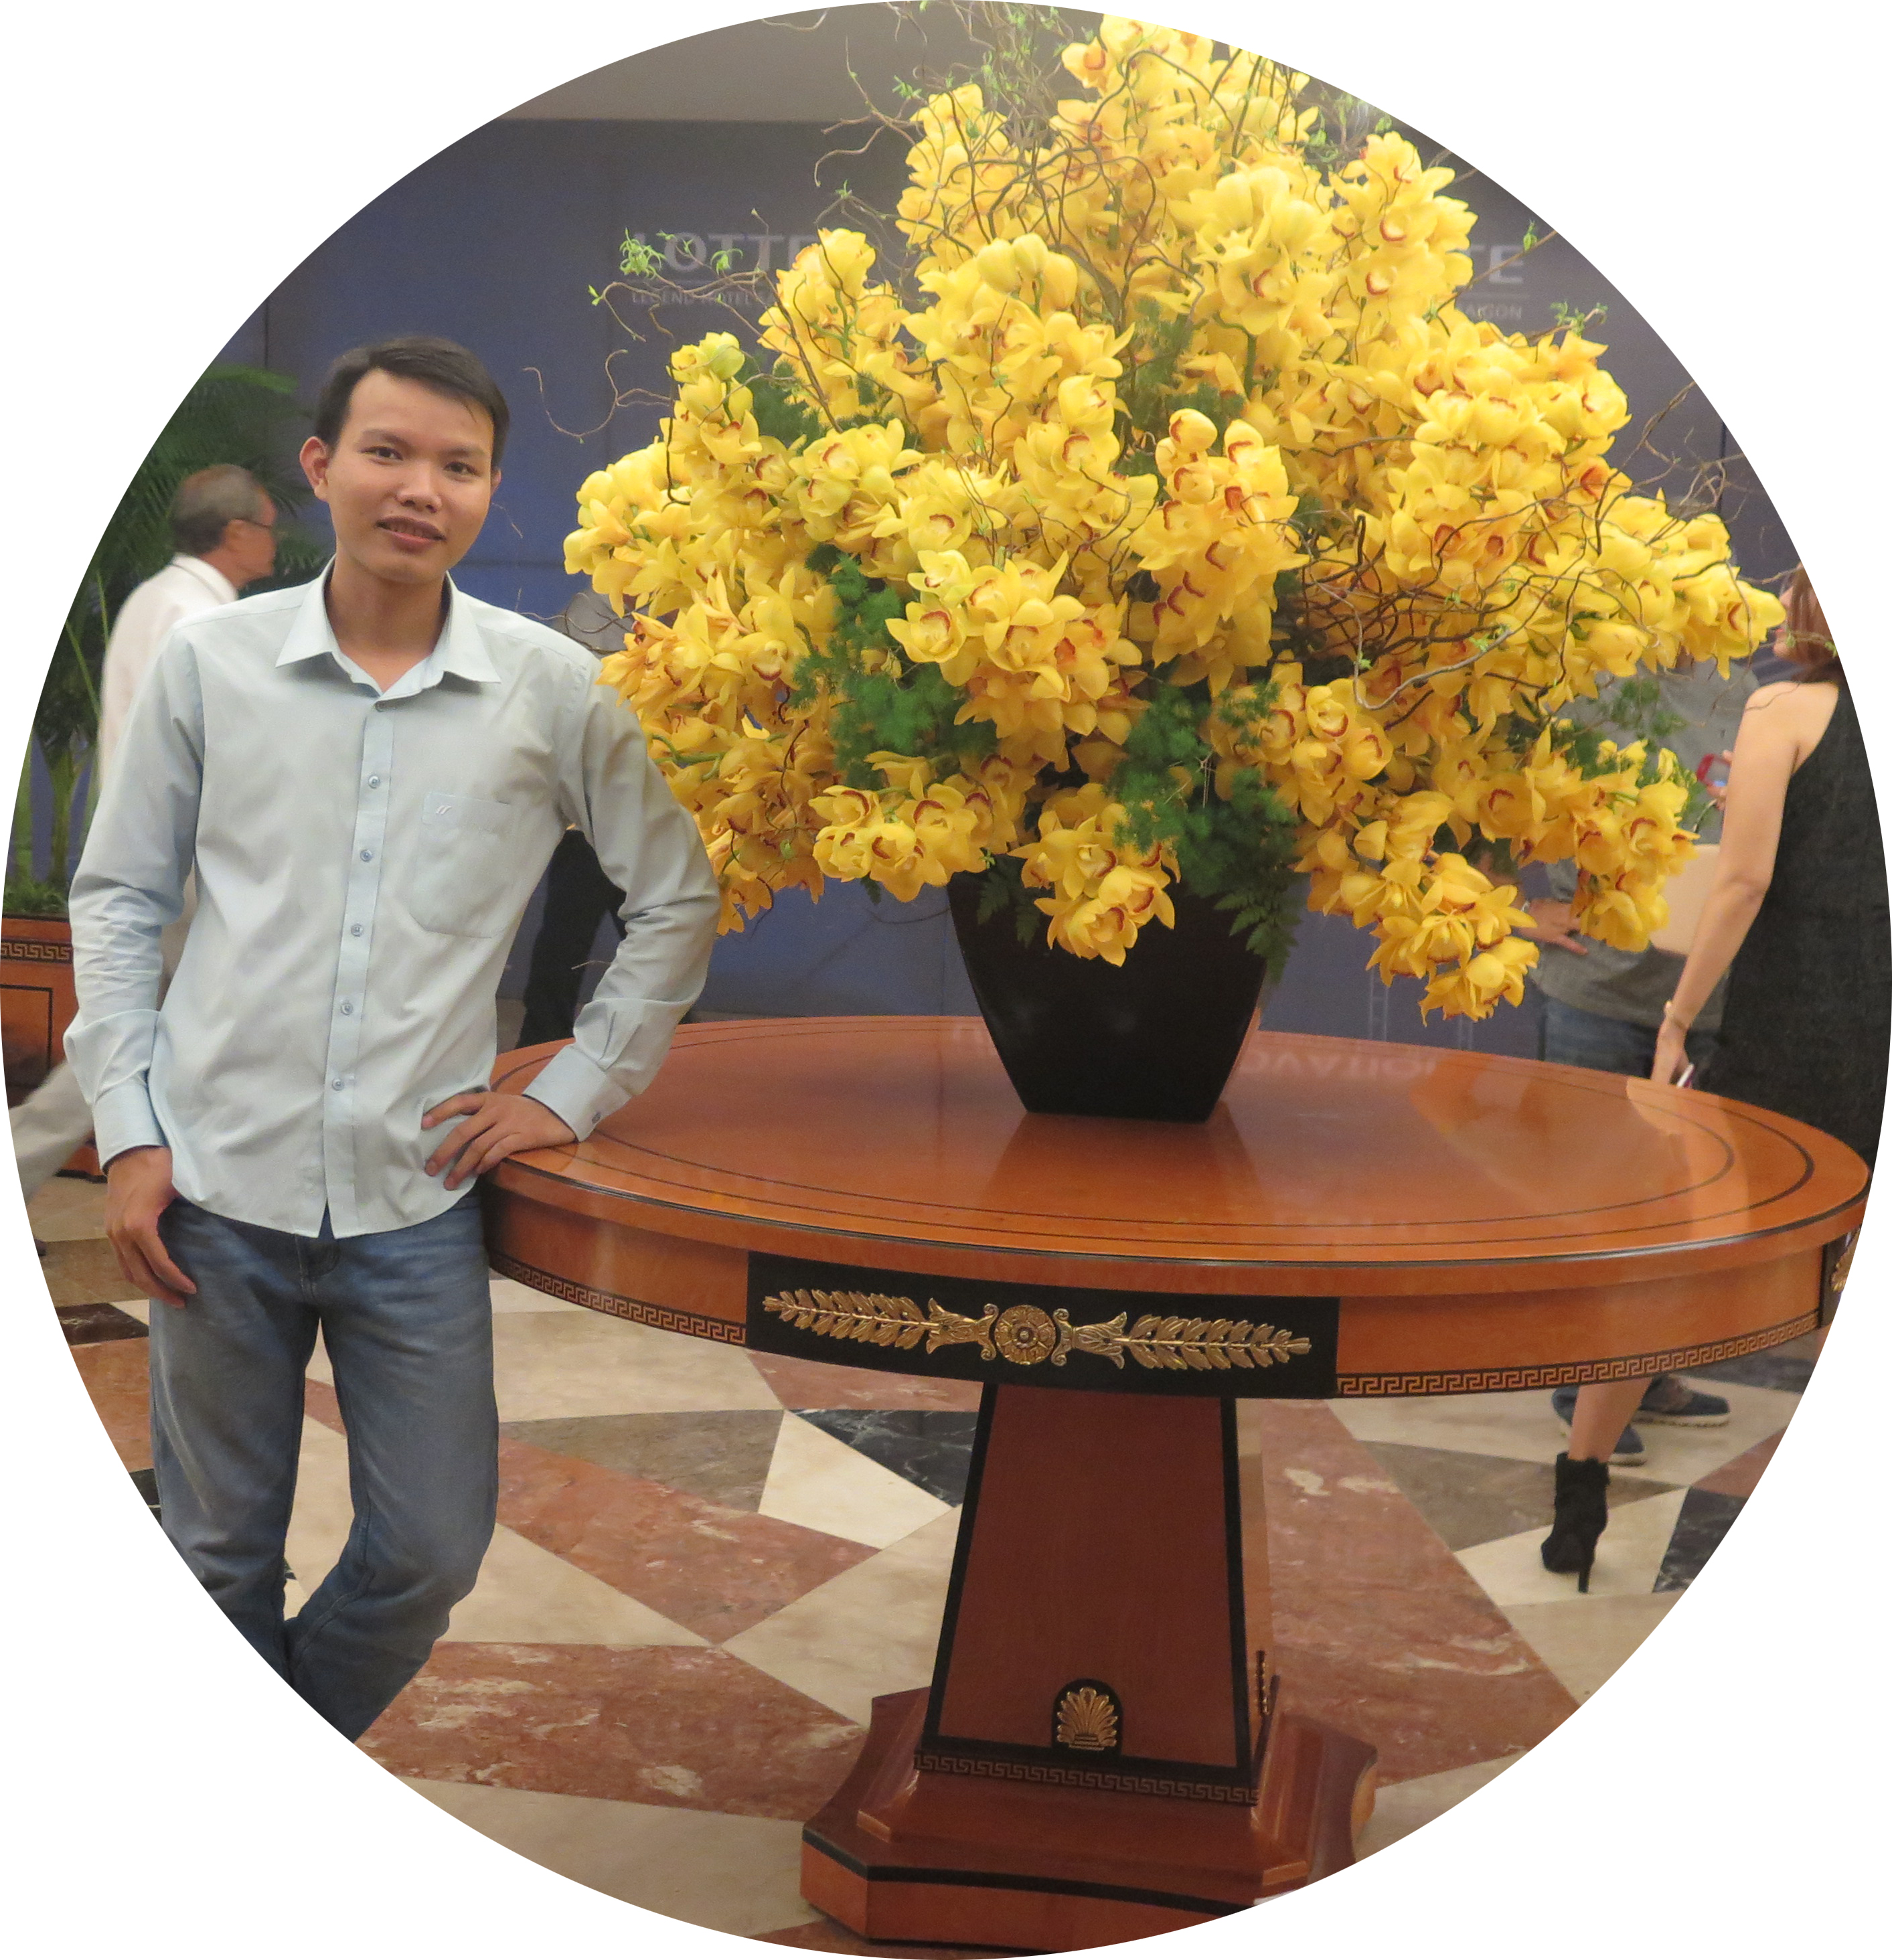
\includegraphics[scale=0.1]{img/kalog-noedit.jpg}
   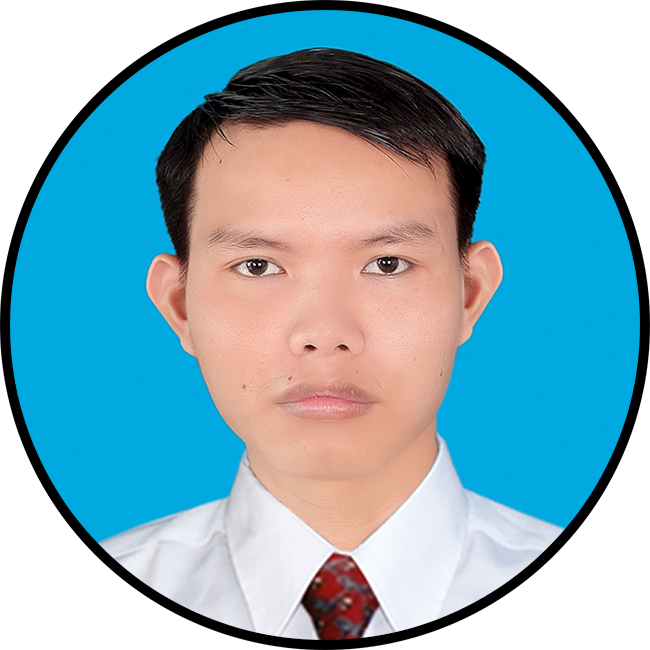
\includegraphics[scale=0.8]{img/circle01.jpg}
  \section{Full Name}
Nguyen Quoc Long
  \section{Gender}
Men
  \section{Date of birth}
    %\href{mailto:longnguyencse@gmail.com}{\textbf{longnguyencse@}\\gmail.com}\
	18/05/1993
~
~
~
  % use  \hspace{} or \vspace{} to change bubble size, if needed
  \section{Programming}
~
    \smartdiagram[bubble diagram]{
        \textbf{Java},
        \textbf{Python},
        \textbf{C/C++},
        \textbf{JS},
        \textbf{PHP}
    }
~
~
  \section{Personal Skills}
~
    \smartdiagram[bubble diagram]{
        \textbf{Team}\\\textbf{Player},
      %  \textbf{Initiative}, % sang kien
        \textbf{Curiosity}, % ham hieu biet
        \textbf{Problem}\\\textbf{Solving},
        \textbf{Manage},
        \textbf{Organize}
    }
    ~
\end{aside}
~


%\begin{aside}
%~
%~
%~
%  \section{OS Preference}
%    \textbf{GNU/Linux}
\includegraphics[scale=0.40]{img/4stars.png}
%    %\textbf{Unix}
\includegraphics[scale=0.40]{img/4stars.png}
%    \textbf{MacOS}
\includegraphics[scale=0.40]{img/1stars.png}
%    \textbf{Windows}
\includegraphics[scale=0.40]{img/4stars.png}
%   % ~
%  %\section{Places Lived}
%    %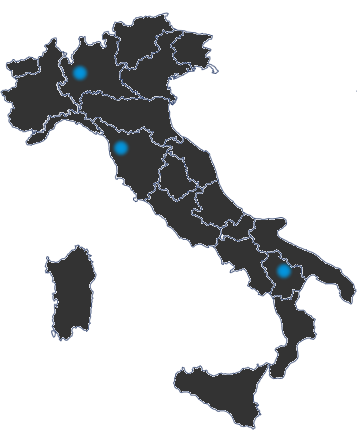
\includegraphics[scale=0.25]{img/italia.png}
%    %~
%  \section{Languages}
%    \textbf{Vietnamese}
\includegraphics[scale=0.40]{img/5stars.png}
%    \textbf{English}
\includegraphics[scale=0.40]{img/2stars.png}
%    ~
%\end{aside}
%\hspace{1cm}  \textbf{Summary Object}: Looking to leverage my knowledge and experience into a role~
%\hspace{3cm} 

%			 \textbf{\hspace{6cm}  as application development specialist}\\
%\section{Summary Object:}
\begin{entrylist}
	\hspace{0.5cm} \info{Summary Object: }{ Looking to leverage my knowledge and experience into a role  as\\ application development specialist}
\end{entrylist}
\begin{center}
\section{Person Information}
\end{center}
%\begin{entrylist}
%\info{Address: }{Tan Binh District, Ho Chi Minh City, Viet Nam}
%\info{Email:}{longnguyencse@gmail.com}
%\info{Contact tel:}{+84 93 246 7086}
%\info{Web:}{longbkitblog.wrodpress.com}
%\info{Github:}{https://github.com/longnguyencse}
%\end{entrylist}

\begin{entrylist}
		\hspace{2cm} 	 \info{				Address: }{Tan Binh District, Ho Chi Minh City, Viet Nam}
		\hspace{2cm} 	\info{				Email:}{longnguyencse@gmail.com}
		\hspace{2cm} 	\info{				Contact tel:}{+84 93 246 7086}
		\hspace{2cm} 	\info{				Web:}{longbkitblog.wrodpress.com}
		\hspace{2cm} 	\info{				Github:}{https://github.com/longnguyencse}
\end{entrylist}

\section{Experience}

%\begin{entrylist}
%  \entry
%    {09/15 - 11/15}
%    {Java Developer}
%    {Fujinet Systems JSC}
%    {We build web application by Java and Velocity\\}
%\end{entrylist}
\begin{entrylist}
  \entry
    {11/18 - now}
    {JavaScript Developer}
    {Ikorn Solutions}
    {Developing new Kibana visualizations. We made some significant changes to the visualize API and how visualizations are implemented\\

	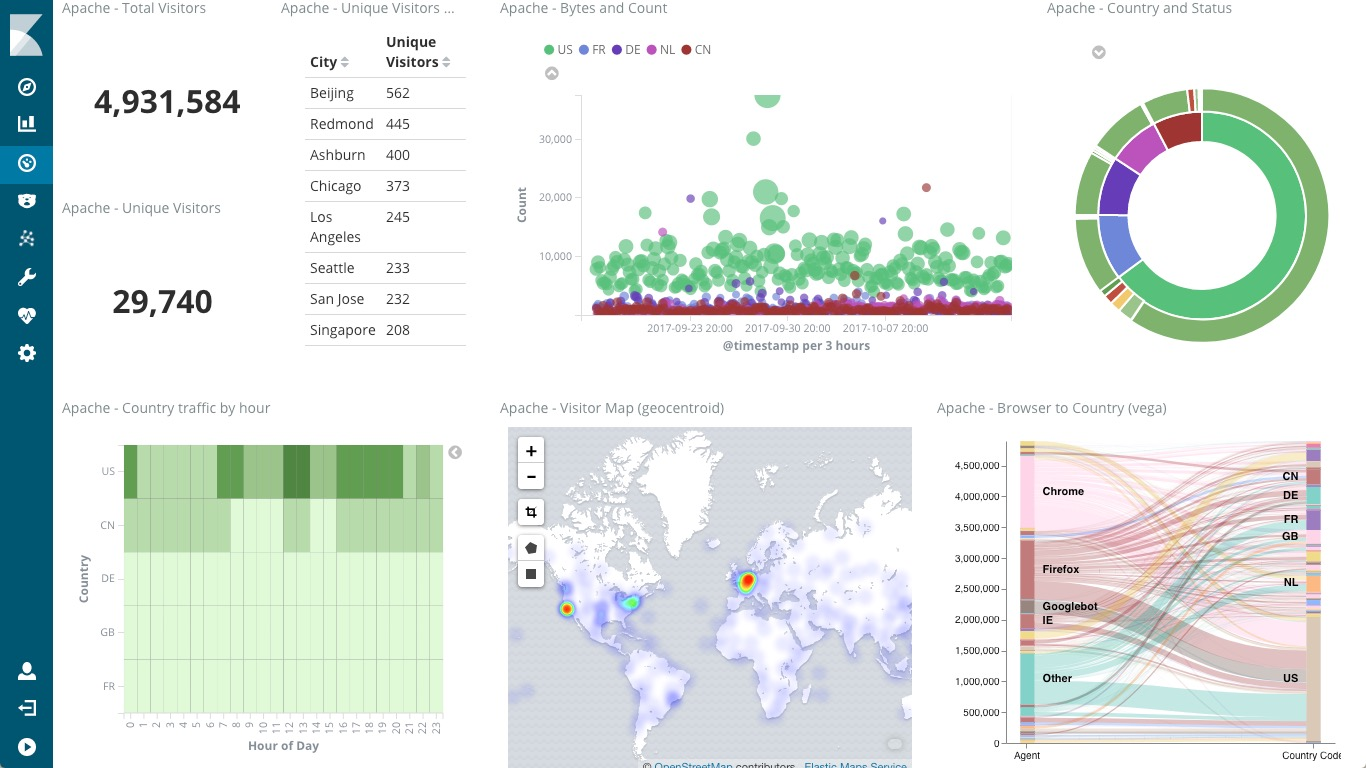
\includegraphics[scale=0.08]{img/kibana_01.jpg} \hspace{2cm}
	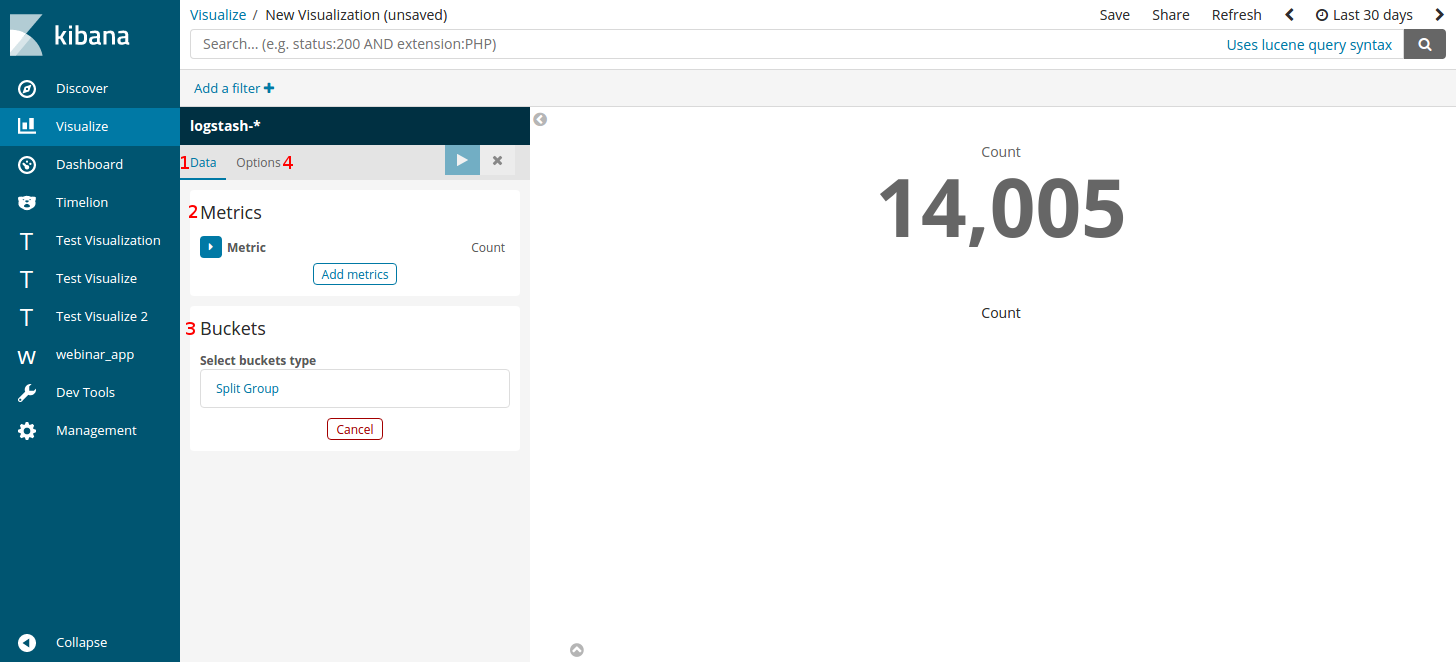
\includegraphics[scale=0.1]{img/kibana.png}\\
	
	\textbf{Development Languages:} PHP/ HTML/ CSS/ JS~\\
	 \textbf{Technologies:}~
			\begin{itemize}
				\item \textbf{Platform:}  Web
				\item \textbf{Framework:} kibana 6.3
				\item \textbf{Protocol:} Http/https
			\end{itemize}
	 \textbf{Engineer Engagement:} 1-2 personnel\\
	 \textbf{Project Duration} 06/2018 - Present~
     }
\end{entrylist}

\begin{entrylist}
\entry
    {11/17 - Now}
    {Java Developer}
    {Ikorn Solutions}
	{\textbf{ Data Annotation: } We label all videos and images that were recorded while driving. This ground truth is the basis for training objects detection algorithms.\\
	We use Apache Kafka, Apache Strom, Apache Hadoop, HDFS, Vert.x and MongoDb to build data lake.\\
		
	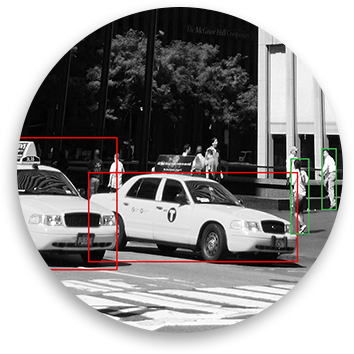
\includegraphics[scale=0.3]{img/labeling_img_14.png} \hspace{1cm}
	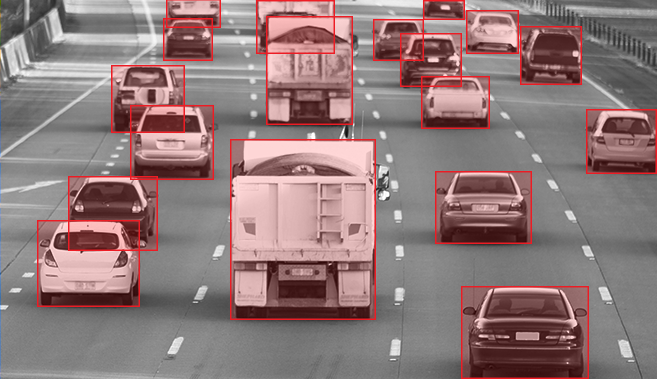
\includegraphics[scale=0.25]{img/labeling_img_5_1.png}\\
}
\end{entrylist}

\begin{entrylist}
\entry
%    {11/17 - Now}
%    {Java Developer}
%    {Ikorn Solutions}
{}
{}
{}
	{ \textbf{Development Languages:} PHP/ HTML/ CSS/ JS~\\
	 \textbf{Technologies:}~
			\begin{itemize}
				\item \textbf{Platform:}  Web, Application
				\item \textbf{Framework:} Kirita, Meteor Js, Apache Nifi,  Vert.x, Apache Storm, Apache Kafka  
				\item \textbf{Database:} MySQL, Apache Solr
				\item \textbf{Protocol:} Http/https
			\end{itemize}
	 \textbf{Engineer Engagement:} 12 personnel\\
	 \textbf{Project Duration} 12/2017 - Present~
	}
\end{entrylist}

\begin{entrylist}
  \entry
    {01/16 -10/17}
    {Java Developer}
    {Ikorn Solutions}
   {\textbf{ Dubu Suite:} We have built multiple applications and communications systems that are widely-used in our target industries.~
	 Many of our systems are designed on modular basic with independent applications that seamlessly dovetail into stable, fully-intergrated packages.\\

	 \textbf{Development Languages:} Java, C++, HTML/CSS/JS\\
	 \textbf{Technologies:}~
			\begin{itemize}
				\item \textbf{Platform:} Web, Window and Mobile
				\item \textbf{Framework:} Spring MVC, Struts
				\item \textbf{Database:} MySQL, NoSQL (Mongo, Mnesia)
				\item \textbf{Protocol:} MySQL, NoSQL (Mongo, Mnesia)
			\end{itemize}
		 \textbf{Engineer Engagement} 16 personnel\\
		 \textbf{Project Duration} 36 months\\
		 \textbf{Component products :} Dubu messenger, Dubu mail, dubu log, dubu sns, dubu disk, dubu editor\\
}
\end{entrylist}

\begin{entrylist}
\entry
    {07/16 - 12/16}
    {Java Developer}
    {Ikorn Solutions}
	{\textbf{ Quark}  is B2B marketplace for marketing affiliate partners with \#Value Links.\\ 
	It is dedicated to connecting the world’s supply chains and accelerating the adoption of sustainable \#Value Links practices.
	With a free account and support for multiple languages, it’s extremely easy to use.\\
	 Just a few simple mouse clicks, and administrator can monitor displayed item views, popularity, and visitor counts.\\
	Quark Clawler is the clawer for collecting data  for QuarkB2B website.\\

	 \textbf{Development Languages:} PHP/ HTML/ CSS/ JS, Java (Web Crawler) \\ 
	 \textbf{Technologies:}~
			\begin{itemize}
				\item \textbf{Platform:} Web,  Mobile, hadoop-hdfs (File system for web clawer)
				\item \textbf{Framework:} Yii, Apache Nutch (Web Clawer)
				\item \textbf{Database:} MySQL, Apache Solr, HBase (Database for Web Clawer)
				\item \textbf{Protocol:} Http/https
			\end{itemize}
		 \textbf{Engineer Engagement:} 11 personnel\\
		 \textbf{Project Duration} 12  months~
	}
\end{entrylist}

\begin{entrylist}
\entry
    {11/15 - 06/16}
    {Java Developer}
    {Ikorn Solutions}
	{\textbf{ Dubu Plus: } A multifunctional responsive web builder that makes it easy to create a website without any professional knowledge.
	\\ This can leverage optimized ecosystems for multiple devices such as PC, tablet, mobile, etc. and offer full support for businesses including shopping and booking packages.\\
}
\end{entrylist}

\begin{entrylist}
\entry
{}
{}
{}
{
		 \textbf{Development Languages:} PHP/ HTML/ CSS/ JS~\\
		 \textbf{Technologies:}~
			\begin{itemize}
				\item \textbf{Platform:} Web,  Mobile
				\item \textbf{Framework:} Custom
				\item \textbf{Database:} MySQL, NoSQL (Mongo, Mnesia)
				\item \textbf{Protocol:} MySQL, NoSQL (Mongo, Mnesia)
			\end{itemize}
		 \textbf{Engineer Engagement:} 10 personnel\\
		 \textbf{Project Duration} 24  months\\
	}
\end{entrylist}

\begin{entrylist}
  \entry
    {09/15 - 11/15}
    {Java Developer}
    {Fujinet Systems JSC}
    {We build web application by Java and Velocity\\}
\end{entrylist}

\begin{entrylist}
    \entry
    {06/14 - 08/14}
    {Java Developer - Intership (Prepoolk24)}
    {FPT Software}
    {We learn software development process (SEP) , using subversion (SVN) and develop web applications using Structs 2 Web framework\\}
\end{entrylist}
%\newpage
\section{Education}
\begin{entrylist}
  \entry
    {2017 - Now}
    {Master's Degree in Computer Engineering}
    {Bach Khoa University}
    {Current enrolled for first years at Back Khoa university. Course taken include: 
Advanced Programming , Advanced Computer Architeture , Advanced Algorithms,…\\}
\end{entrylist}
\begin{entrylist}
  \entry
    {2011 - 2016}
    {Bachelor's Degree in Computer Engineering}
    {Bach Khoa University}
    {Grandted Bachelor of Engineering of Back Khoa University major Computor sience. Cumulative Major GPA 7.29\\
       $*$ \textbf{Intership:} Android system encrypts files by using the biometric facial recognition feature.\\
       $*$ \textbf{Thesis:} 	Workflow management system of factory textile base on web application\\}
\end{entrylist}

%\newpage

\begin{aside}
~
~
~
  \section{OS Preference}
    \textbf{GNU/Linux}
\includegraphics[scale=0.40]{img/4stars.png}
    %\textbf{Unix}
\includegraphics[scale=0.40]{img/4stars.png}
    \textbf{MacOS}
\includegraphics[scale=0.40]{img/1stars.png}
    \textbf{Windows}
\includegraphics[scale=0.40]{img/4stars.png}
   % ~
  %\section{Places Lived}
    %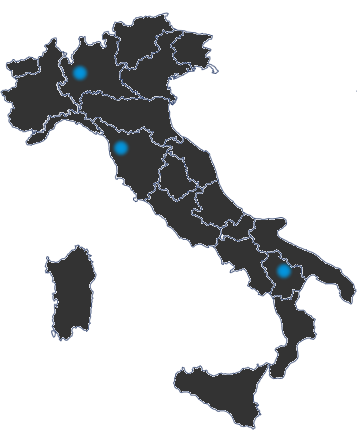
\includegraphics[scale=0.25]{img/italia.png}
    %~
  \section{Languages}
    \textbf{Vietnamese}
\includegraphics[scale=0.40]{img/5stars.png}
    \textbf{English}
\includegraphics[scale=0.40]{img/2stars.png}
    ~
\end{aside}

\section{Volunteer Experience}
Student Volunteer\\
\textbf{Support the activities of the holiday season in Phật Quang Pagoda - Vũng Tàu}\\
\emph{Visit SOS Children's Village (Đông Hòa, Dĩ AN, Bình Dương)}
\\
%\section{Honors \& Awards}
%\begin{entrylist}
  %\entry
  %  {10/2015}
  %  {Best swordsman duel}
  %  {Contest}
  %  {Lorem ipsum.\\
  %  \emph{Lorem ipsum}}
%\end{entrylist}

\section{Certifications}
\begin{entrylist}
  \entry
    {06/2015}
    {TOEIC}
    {IIG Vietnam}
    {\emph{Test of English for International Communication}}
\end{entrylist}

%\section{Other Info}
%For the Italian job market:\\
%\emph{Si autorizza il trattamento delle informazioni contenute nel curriculum in conformità alle disposizioni previste dal %d.lgs. 196/2003. Si dichiara altresì di essere consapevole che, in caso di dichiarazioni non veritiere, si è passibili di sanzioni %penali ai sensi del DPR 445/00 oltre alla revoca dei benefici eventualmente percepiti.}
%\\
\begin{flushleft}
\emph{Jul 17th, 2018}
\end{flushleft}
\begin{flushright}
\emph{Long Nguyen}
\end{flushright}

\end{document}
